\documentclass[sigconf]{acmart}
%%
%% \BibTeX command to typeset BibTeX logo in the docs
\AtBeginDocument{%
  \providecommand\BibTeX{{%
    \normalfont B\kern-0.5em{\scshape i\kern-0.25em b}\kern-0.8em\TeX}}}

%% These commands are for a PROCEEDINGS abstract or paper.
\setcopyright{none}
\settopmatter{printacmref=false}
\renewcommand\footnotetextcopyrightpermission[1]{}
\acmConference[ECE595SE]{ECE595: Advanced software engineering}{February 2021}{West Lafayette, IN, USA}
\acmPrice{00.00}
\acmISBN{978-1-4503-XXXX-X/18/06}

\usepackage[
    backend=biber,
    style=ieee,
  ]{biblatex}
\addbibresource{references.bib}
\usepackage{rotating}
\usepackage{multirow}

\begin{document}

%%
%% The "title" command has an optional parameter,
%% allowing the author to define a "short title" to be used in page headers.
\title{A Reproduction of ``DeepBugs: A Learning Approach to Name-based Bug Detection"}

%%
%% The "author" command and its associated commands are used to define
%% the authors and their affiliations.
%% Of note is the shared affiliation of the first two authors, and the
%% "authornote" and "authornotemark" commands
%% used to denote shared contribution to the research.
\author{Caleb Tung}
\affiliation{%
  \institution{Purdue University}
  \city{West Lafayette}
  \state{Indiana}
  \country{USA}}
\email{tung3@purdue.edu}

\author{Dario Rios Ugalde}
\affiliation{%
  \institution{Lockheed Martin}
  \city{Arlington}
  \state{Texas}
  \country{USA}}
\email{dugalde@purdue.edu}

\author{Young Jin Jung}
\affiliation{%
 \institution{Purdue University}
 \city{West Lafayette}
 \state{Indiana}
 \country{USA}}
\email{jung199@purdue.edu}

\author{Jordan Matthew Winkler}
\affiliation{%
 \institution{Purdue University}
 \city{West Lafayette}
 \state{Indiana}
 \country{USA}}
\email{jwinkler@purdue.edu}

\author{Abhimanyu Agarwal}
\affiliation{%
  \institution{Purdue University}
  \city{West Lafayette}
  \state{Indiana}
  \country{USA}}
\email{agarw184@purdue.edu}
%%
%% By default, the full list of authors will be used in the page
%% headers. Often, this list is too long, and will overlap
%% other information printed in the page headers. This command allows
%% the author to define a more concise list
%% of authors' names for this purpose.
\renewcommand{\shortauthors}{Caleb et al.}

%%
%% The abstract is a short summary of the work to be presented in the
%% article.
\begin{abstract}
\label{sec:abstract}

INTRODUCTION: Reproducibility and replication of existing work is important in the research community. For works that are not reproduced, the validity of the work may be questioned, since the results are unvalidated. The research community has labeled the large amount of unreproduced work as the  ``reproducibility crisis''. Researchers often do not undertake replication studies because there are relatively few incentives to do so.
In this project, we replicate \textit{DeepBugs} by Pradel and Sen, a novel automated name-based bugs detection framework. We re-implement the DeepBugs algorithm from scratch and test it with the original dataset, verifying the original authors' claims.
STATE-OF-ART: The research community is encouraging more replication studies, with journals and workshops dedicated to replication work. Prior to this paper, there were no replication studies for DeepBugs. CONTRIBUTION: In this project, we perform a replication study of the DeepBugs name-based bug detection framework. This provides validation for those who wish to implement DeepBugs into their work. METHOD: We re-implement the DeepBugs artifacts for training set generation, source code vectorization, and neural network training and testing. The team uses Python, while the original work uses mostly JavaScript. RESULTS: The team successfully replicated DeepBugs by following the process outlined in the original work. The resulting reimplementation of the framework has an accuracy only 2\% lower than that of the original.
\end{abstract}


\begin{CCSXML}
<ccs2012>
   <concept>
       <concept_id>10011007.10011006.10011073</concept_id>
       <concept_desc>Software and its engineering~Software maintenance tools</concept_desc>
       <concept_significance>500</concept_significance>
       </concept>
 </ccs2012>
\end{CCSXML}

\ccsdesc[500]{Software and its engineering~Software maintenance tools}

%%
%% Keywords. The author(s) should pick words that accurately describe
%% the work being presented. Separate the keywords with commas.
\keywords{defect detection, deep learning}

%%
%% This command processes the author and affiliation and title
%% information and builds the first part of the formatted document.

\maketitle

\section{Introduction}

In this project, we will perform a replication study of \textit{DeepBugs: A Learning Approach to Name-based Bug Detection} \cite{pradel_deepbugs_2018}. We select this paper because (1) our team is interested in automated bug detection methods, and (2) the paper is particularly novel when compared to other automated bug detectors. Instead of using hand-crafted heuristics to judge where source code contains bugs, the DeepBugs framework fully automates the detection of name-based bugs via deep learning. Moreover, since the paper first appeared in a 2018 OOPSLA issue of \textit{The Proceedings of the ACM on Programming Languages}, it has gained considerable popularity. According to the ACM, 40 other peer-reviewed works cite the paper, while Google Scholar registers the total citation count at 99.

In our replication study, we will implement the algorithms outlined in the DeepBugs paper and test them using the original authors' data sets to see if we can reproduce the same results. 



% Neural networks are tight!

% TODO: move future tense to past tense

\section{Motivation}
\label{sec:introduction}
In a 2016 survey by Springer \cite{baker_1500_2016}, 52\% of scientists across multiple fields of study reported that they felt there was a ``significant crisis'' in the reproducibility of published research. Another 38\% felt there was a ``slight crisis.'' This ``reproducibility crisis'' describes the consensus among the scientific community that an outsized portion of published research is not reproduced. ``Our analysis...suggests
a large proportion of CS research faces
the same threats to replication as those
encountered in other areas,'' writes Cockburn, et al in a recent edition of \textit{Communications of the ACM}. Non-reproducible research is problematic because (1) it is more challenging for other researchers to use the research technology in their own projects, and (2) there exists no independent verification of the research's validity. Therefore, reproducing research should be important to the scientific community. 

\begin{figure}
    \centering
    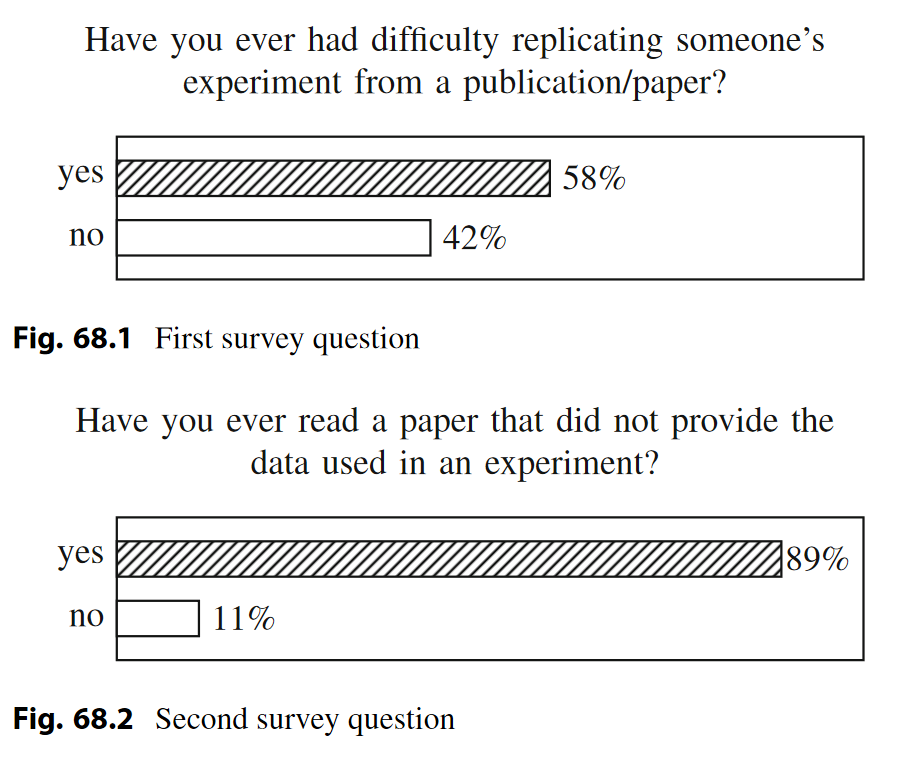
\includegraphics[width=\linewidth]{images/IT.PNG}
    \caption{ (image credit ITNG 2020 \cite{cacho_state_2020})}
    \label{fig:nature_magazine_reproducibility_figure}
    \vspace{-0.2in}
\end{figure}

Unfortunately, few replication studies (formal studies that attempt to independently reproduce an existing work and document its results) are attempted. This is due to many reasons, including: reproducing a study might be expensive, attempting to question an author might be seen as malicious or reflecting incompetence, spending the time to reproduce a study may not further one's own research, etc. Additionally, scientists unable to reproduce work might be inclined to write off a failure as some personal mistake and move on. Incentives to publish positive replications are already low; journals can be even more reluctant to publish negative findings \cite{cacho_state_2020}. This all contributes to the ``file drawer effect'': replication work that would otherwise be useful goes unpublished \cite{cockburn_threats_2020}.  Therefore, the lack of replication studies continues.
% ``When work does not reproduce, researchers often assume there is a perfectly valid (and probably boring) reason. What's more, ,'' writes \textit{Nature} editor Monya Baker \cite{baker_1500_2016}. T

 By performing the replication study ourselves, we wished to contribute to the software engineering community and add a positive effect to mitigate the ``reproducibility crisis.'' Hopefully, our replication study motivates other software engineers to participate in replication studies. Narrowly, we attempt to give a better insight to other researchers who seek to implement DeepBugs into their system. 

\section{Background and Related Work}
\label{sec:background_and_related_work}

% \textbf{TODO!!!! Make sure the 5 papers we asses end up discussed here too}

% Dario [X]
% https://dl.acm.org/doi/pdf/10.1145/3379597.3387491 (How Often Do Single Statement Bugs Occur)

% Caleb [X]
% https://www.sciencedirect.com/science/article/pii/S0950584917304305 (The role and value of replication in empirical software engineering results)

% Abhimanyu []
% https://citeseerx.ist.psu.edu/viewdoc/download?doi=10.1.1.91.8408&rep=rep1&type=pdf (D. Hovemeyer, J. Spacco, and W. Pugh, “Evaluating and tuning a static analysis to find null pointer bugs")

% Jordan [X]
% https://dl.acm.org/doi/10.1145/2884781.2884841 (Nomen est omen: exploring and exploiting similarities between argument and parameter names)

% Young []
% https://dl.acm.org/doi/pdf/10.1145/3183519.3183525 (Modern Code Review: A Case Study at Google) :^} XOR https://dl.acm.org/doi/pdf/10.1145/1287624.1287634 (Context-Based Detection of Clone-Related Bugs)



%\textbf{FINAL REPORT TODO!!!! Explain what name-related bugs are, what the switched argument bug is and how it cannot be detected by conventional methods}

% done 

% \textbf{TODO!!!! Go through Prof. Davis' Background/Related Work comments to be sure we got everything}

% done

%\textbf{TODO!!!! Talk about why replication studies are important}

% wasn't this done in motivation? And then it is done a few times in ethics. Does it need to be done again here?


\subsection{Automated bug detection}
\label{subsec:deepbugs_related_work}
Automated bug detection is an active area of research. There is a wealth of statistical information in identifier names. \cite{liu_nomen_2016} DeepBugs specifically addresses name-based bug detection unlike several popular static analysis tools, such as Google Error Prone \cite{aftandilian_building_2012} and FindBugs \cite{hovemeyer_evaluating_2005} that mostly ignores identifier names. Name-based bugs are bugs that can be tracked by linguistic similarity. An example of this is the association of the variable $x$ with width and $y$ with height. In a program, this could lead to a switch-argument bug. Switch-argument bugs are part of a class of bugs called single-statement bugs, which have been reported to consist possibly as much as 33\% of bugs in some Java projects. \cite{karampatsis_how_2020}

The reason many program analysis tools ignore identifier names is because such detection is challenging. Name-based analysis must encode the meaning of identifier names, which can be based on subconscious cultural knowledge. Although lexical reasoning is often used to achieve this, existing name-based analysis relies on manually designed algorithms that use hard-coded patterns and tuned heuristics which require significant amount of time and human effort \cite{host_debugging_2009, noauthor_nomen_nodate, pradel_deepbugs_2018, noauthor_detecting_nodate}. In contrast, DeepBugs uses a deep learning approach to detect bugs automatically. This is done by training the neural network on a large corpus of code examples.

Before the identifiers can be trained on, they must first be extracted from code. Conditional random fields and statistical machine translation have been used to do this in works such as JSNice \cite{raychev_predicting_2015} and JSNaughty \cite{vasilescu_recovering_2017}. DeepBugs used Word2Vec \cite{mikolov_efficient_2013} to automatically generate vector representations of code snippets to feed into a neural network. Furthermore, in contrast to previous work, DeepBugs focused on implicitly typed languages, where information about the code semantics is conveyed through identifier names by programmers instead of types. The overall framework complements any designed bug detector that relies on processes inducing significant manual work, thereby replacing human effort by transitioning to computational means to achieve the same. 

\subsection{Similar models for analyzing and finding bugs}
\label{subsec:Models for Analyzing and Finding Bugs}

The DeepBugs model learns from positive examples and negative examples, focusing on bug patterns that can be expressed via probabilistic means. On the other hand, Bugram \cite{wang_bugram_2016} uses an n-gram model of code to detect bugs with positive examples only (i.e., anomaly detection). Specification mining \cite{ammons_mining_2002} uses mined features and specifications to detect unusual bugs in code \cite{liang_antminer_2016,pradel_deepbugs_2018,wasylkowski_mining_2011} while learning only from correct examples and flagging any inconsistencies and errors. 

While DeepBugs finds bugs and pinpoints the bug location, Wang, et al.'s approach uses a deep belief network \cite{wang_automatically_2016}  to flag buggy code files for further inspection. Ultimately, DeepBugs differs from existing name-based bug detectors in that it (1) exploits semantic similarities that may not be identified by lexical comparison of identifies, (2) improves generalizability by replacing manually tuned heuristics with a deep neural network.

\subsection{Background on replication studies}
\label{subsec:background_on_replication_studies}


According to the ACM, replication of an existing study should be performed by a ``different team, with the same experimental setup" \cite{noauthor_artifact_nodate}. And according to BSEL, complete reporting is also highly important due to possible high variance of the parameter of interest. \cite{shepperd_role_2018} More concretely, the replication study should be conducted without deploying the original authors' artifacts and should instead use independently generated artifacts. The original study is verified if those new artifacts achieve the same results as those found in the original paper. A reproduction study differs from a replication study: a reproduction study checks whether the original results can be obtained using the author's artifacts, while a replication study requires the artifacts to be generated from scratch. Our study will reuse the original authors' code data set \cite{pradel_michaelpradeldeepbugs_2021} but will implement the DeepBugs algorithms using our own source code. Therefore, our project would qualify as a replication study.

It is worth noting that replication studies remain largely unwelcome in academic venues; for example, only 3\% of 1,500 top psychology journals welcome replication work as submissions \cite{martin_are_2017}. Fortunately, in recent years, a few research communities have tried to increase incentive for replication studies. Targeted at software engineering research, the ROSE Festival exclusively features replication work \cite{noauthor_rose_nodate}. Similarly, the Association for Information Systems publishes an entire journal, \textit{Transactions on Replication Research}, dedicated to reproducibility studies \cite{noauthor_ais_nodate}.

Our replication study of DeepBugs will be unique; to our knowledge, there exists no such study for that work.
\section{Reimplementing DeepBugs}
\label{sec:replicating_deepbugs}

DeepBugs is structured as shown in Fig. \ref{fig:deepbugs-overview}. DeepBugs first converts a piece of source code (their source code is taken from the 150k JavaScript Dataset \cite{noauthor_150k_nodate}) into an Abstract Syntax Tree (AST). %AST is probably public domain knowledge by now, no worries about citation
The tree is parsed and converted into condensed tokens that represent the relevant code symbols. The symbols are then turned into vectors so that they can be passed into a neural network to classify if the code is buggy or not.

\begin{figure}[h]
    \centering
    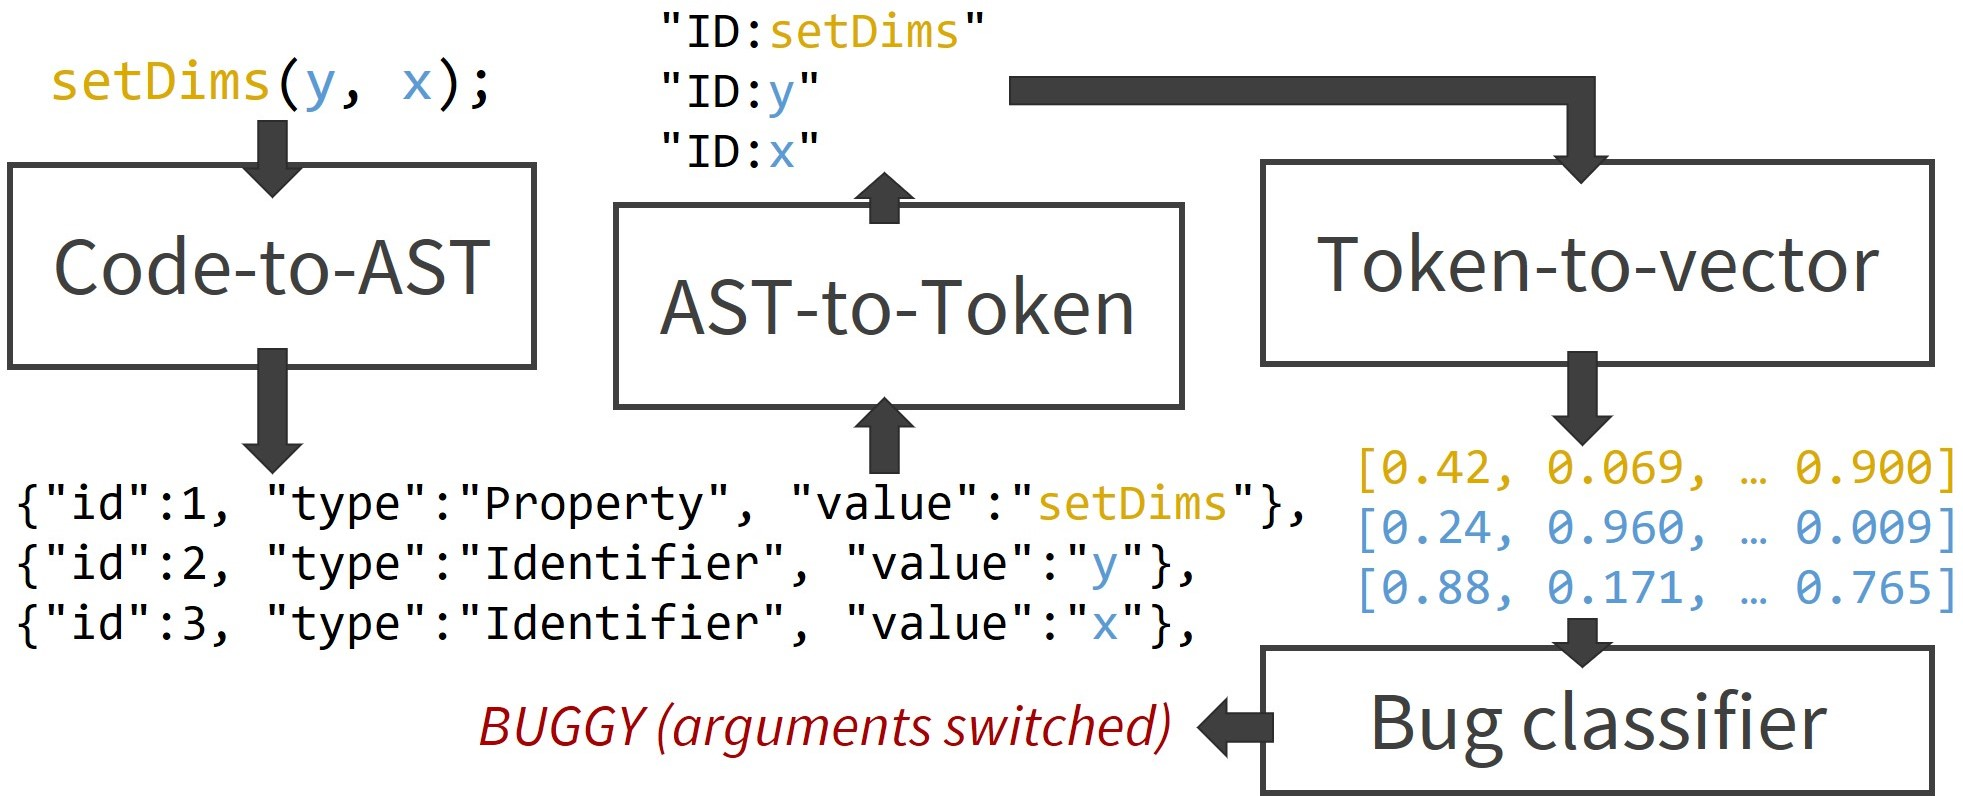
\includegraphics[width=\linewidth]{images/deepbugs-overview.jpg}
    \caption{DeepBugs first converts source code into Abstract Syntax Trees (ASTs) and then into semantic-encoded vectors. The vectors are input to a deep learning model that determines if the source code is buggy. Here, a developer has written a function call for \texttt{setDims(width, height)} using \texttt{setDims(y, x)}. DeepBugs predicts this as ``buggy'' because the system understands that \texttt{x, width} are semantically similar, as are \texttt{y, height}. Thus, it predicts the arguments are swapped; the order should be \texttt{(x, y)}, not \texttt{(y, x)}.}
    \label{fig:deepbugs-overview}
\end{figure}

The DeepBugs framework is designed to detect any name-based bug pattern. Like the original authors, we implement the framework for the ``swapped argument'' bug case. Our reimplementation of DeepBugs is described in the following four steps.

\subsection{Step 1: Code-to-AST}
\label{subsec:step-1}
The original authors used the Acorn JavaScript parser \cite{noauthor_acornjsacorn_2021} to convert JavaScript source code files into a Json formatted Abstract Syntax Tree (AST). For simplicity of testing the swapped-argument bug pattern, we removed AST nodes unrelated to name-base bugs. Our simplified format only uses the \texttt{``children''} AST attribute, which identifies the AST nodes that are acted upon by a given statement or call block. For example, calling some method \texttt{object.methodName(arg1, arg2)} would yield the following simplified AST structure:
\\

\small
\texttt{\{``id'':1, ``type'':``CallExpression'', ``children'':[2,5,6]\},}

\texttt{\{``id'':2, ``type'':``MemberExpression'', ``children'':[3,4]\},}

\texttt{\{``id'':3, ``type'':``Identifier'', ``value'':``object''\},}

\texttt{\{``id'':4, ``type'':``Property'', ``value'':``methodName''\},}

\texttt{\{``id'':5, ``type'':``Identifier'', ``value'':``arg1''\},}

\texttt{\{``id'':6, ``type'':``Identifier'', ``value'':``arg2''\}}\\

\normalsize

This allows us to quickly switch the ordering of the elements in the \texttt{``children''} list and generate swapped-argument bugs.

\subsection{Step 2: AST-to-Token}
\label{subsec:step-2}
For a given bug pattern, not every node in the AST necessarily needs to be evaluated. Further, since each node contains many characters dedicated to represent the node's schema, each relevant group of nodes should be compressed into small tokens that represent the entire group. The tokens can then be vectorized and fed to a neural network for bug classification.

More concretely, for the swapped-argument bug pattern, we are only interested in function names and argument names for any 2-argument function call. To generate tokens, we do the following: For a given AST node, only attempt to generate a token from its \texttt{value} field. If the node does not have a \texttt{``value''} field, derive one from its \texttt{``children''}. The rules we use to generate tokens are similar to those used by the original authors:

\begin{itemize}
    \item A \texttt{CallExpression} with multiple \texttt{Identifier} children can be tokenized separately, with the first child tokenized as the function name, and the remaining children tokenized as the arguments.
    \item A \texttt{MemberExpression} with both an \texttt{Identifier} child and a \texttt{Property} child can be tokenized into the object name and the method/property name, respectively.
    \item Variable names and function names are tokenized as identifiers, with \texttt{``ID:<variable name here>''}.
    \item JavaScript literals of all types are tokenized as 
    \texttt{``LIT:<value>''}.
    \item Other language elements like operands, \texttt{if/else} blocks, \texttt{try/catch} blocks, and \texttt{for} loops are ignored.
\end{itemize}

Using that system, we crawl the entire corpus of code in the 150k JavaScript Dataset, converting each file's AST into a list of tokens. This dramatically compresses the size of our data, distilling only important components. For example, the 6-node AST provided in the Step 1 example (Sec. \ref{subsec:step-1}) would be tokenized into the following list:

\small
\texttt{[``ID:object'', ``ID:methodName'', ``ID:arg1'', ``ID:arg2'']}.
\normalsize

\subsection{Step 3: Token-to-Vector}
\label{subsec:step-3}
To vectorize a token for the neural network bug classifier, the original authors use the Word2Vec \cite{mikolov_efficient_2013} model. Word2Vec can capture lexical similarities between two words, based on the context of the other words surrounding the two words. For example, the letter \texttt{x} and the word \texttt{width} do not necessarily carry similarities on their own. However, in the context of \texttt{setDims()}, they take on similar meanings (i.e., ``width along x-dimension''). Under the CBOW (Collected Bag Of Words) variant, Word2Vec considers a window of words both before and after the word in question to decide the word's vector representation. In our example, this would mean that Word2Vec's output vectors for \texttt{``ID:x''} and \texttt{``ID:width''} would be similar.

To build our Word2Vec model, we first use our AST-to-Token extractor from Step 2 (Sec. \ref{subsec:step-2}) to list all tokens, in order of appearance, for a given JavaScript file's AST. The list of tokens can then be used as a ``paragraph'' of words to feed Word2Vec. We then implement and train our CBOW Word2Vec instance using a window size of 200 tokens (i.e., 100 tokens before the current token, 100 tokens after the current token). To sanity-check our model, we compare the vector similarities of  \texttt{``LIT:true''} with \texttt{``LIT:false''}, \texttt{``LIT:0''}, and \texttt{``LIT:1''} using cosine distance (dot product). We observe that the two true-values are similar to each other (i.e., distance is close to 0), and the two false-values are similar to each other. Meanwhile, the true-values are not similar to the false values (i.e., distance is much farther than 0). This is expected behavior, suggesting that the Word2Vec model is reasonably trained.

\subsection{Step 4: Bug Classifier}
\label{subsec:step-4}
As shown in Fig. \ref{fig:deepbugs-nn}, the DeepBugs bug classifier is a simple neural network that feeds the input through a 20\% dropout regularization layer, a 200-node hidden layer with ReLU activations, another 20\% dropout layer, and a final sigmoidal node to determine the buggy/not buggy prediction. The small size of the network facilitates faster training for different bug patterns.

\begin{figure}[h]
    \centering
    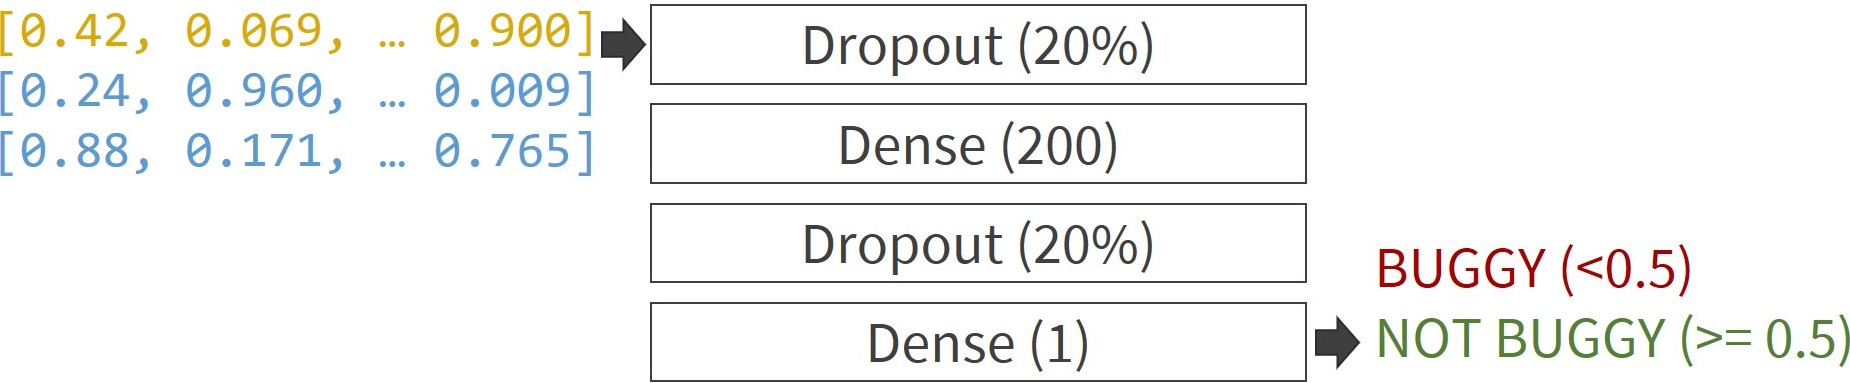
\includegraphics[width=\linewidth]{images/deepbugs-nn.jpg}
    \caption{The Deepbugs classifier is a small neural network that can be rapidly retrained to predict different name-based bugs. As shown, we train our replicated classifier for swapped-argument bug detection.}
    \label{fig:deepbugs-nn}
\end{figure}

Depending on the bug pattern being tested for, the input to the neural network may differ. For the swapped-argument bug, the vectors for the function name and two arguments are concatenated before feeding into the network.



% \section{Experimental Setup}

% \subsection{Problem Statement}
% \label{sec:problem_statement}
% For published research papers, particularly popular ones, it is important for the community to reproduce or replicate the work, thus confirming the validity of the authors' claims.
% Despite being cited repeatedly in the ``Background'' section of other works (DeepBugs has been cited 99 times, according to Google Scholar), DeepBugs has not, to our knowledge, been replicated. Thus, it remains unverified.

% To verify the work detailed by the authors of DeepBugs, we will attempt to replicate their methods. In keeping with the ACM's definitions of ``replication,'' \cite{} if we can implement the algorithms outlined in the DeepBugs paper, run them on the authors' data, and achieve the the authors' 68\% true-positive rate, we will consider our project a success (DeepBugs paper verification is complete).

% If we are unable to achieve the authors' results, we will perform a line-by-line analysis of our implementation. If we cannot find discrepancies between our work and the DeepBugs paper, we will still consider our project a success (DeepBugs paper cannot be verified and should be scrutinized by the community).


% \subsection{Proposed Work}
% \label{sec:proposed_work}
% In this project, we will replicate the DeepBugs paper. As illustrated in Fig. \ref{fig:deepbugs_overview}, the DeepBugs bug detection framework first generates both positive and negative training data from a large dataset of code, then expresses the training data as vectors. A simple binary classifier is then trained; the network's output is either ``TRUE, code is likely bug-free'' or ``FALSE, code likely contains bug.'' Finally, test code can be vectorized and predicted by the neural network. DeepBugs is designed to test for name-based bugs, and the original authors have trained it to identify accidentally swapped arguments and swapped operands.

% \begin{figure}[ht]
%     \centering
%     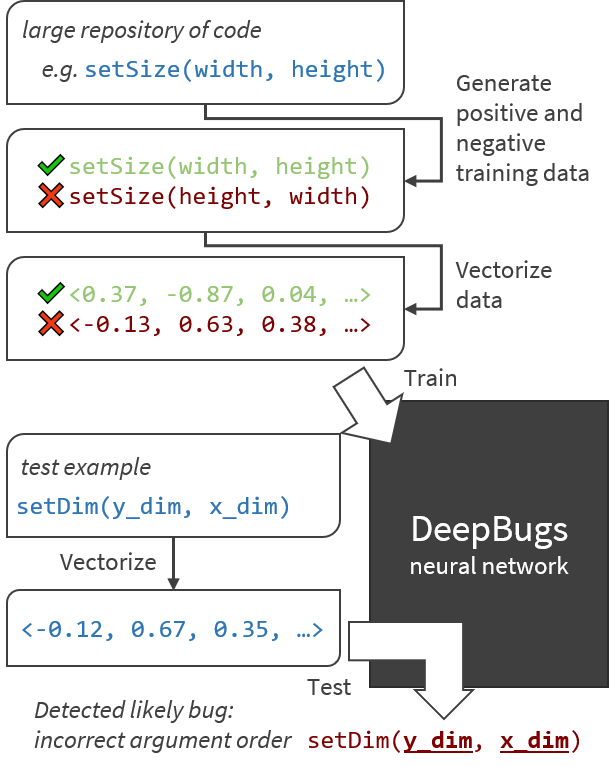
\includegraphics[width=\linewidth]{images/DeepBugs Overview.png}
%     \caption{Overview of the DeepBugs framework.}
%     \label{fig:deepbugs_overview}
% \end{figure}


% \subsection{Generate training data}
% \label{subsec:generate_training_data}
% DeepBugs is trained on large amounts of code. For a given snippet of code, we will create a positive training example (not buggy) and a negative training example (buggy). The original authors supply a large corpus of over 150,000 lines of JavaScript code from which to generate training data; we will use the same corpus. However, we will generate the training examples ourselves.

% We will assume that any given snippet of code from the corpus is likely correct, since the code is pulled from stable commits of well-known open source projects. Therefore, we can use the snippet as a positive example and modify it to become the negative example. As in the original paper, we will first generate an Abstract Syntax Tree (AST) for the code, allowing us to represent the code syntactically as a tree. Then, we can apply a simple AST transformation on the code, e.g. switching the arguments, to create the negative snippets. Both positive and negative examples will be shuffled into the larger dataset.

% \textbf{Verification:} We will verify that our training data generation works correctly by running unit tests. We can then verify the original authors' training examples against our own.

% \subsection{Represent code identifiers as vectors}
% \label{subsec:represent_code_identifiers}
% Because the feedforward classification neural network in DeepBugs requires numerical input, we must translate the training code examples into numerical vectors. This is done through a two-stage process:

% (1) \textit{Vocabulary definition.} Because the DeepBugs classifier must have a fixed input size, the authors set the maximum number of tokens (identifiers and literals) in the code to 10,000 (previously demonstrated to be sufficient in other bug detection experiments). As in the paper, we will select these 10,000 tokens from the code corpus in order of popularity; the remaining tokens will be identified as ``unknown.''

% (2) \textit{Vector encoding by semantic similarity}. In order for DeepBugs to identify accidental coding mistakes, it needs to have an abstract understanding of ``what the developer actually meant to do.'' For example, if trained for swapped arguments on the code snippet \texttt{onComplete(error, result)}, DeepBugs should be able to classify \texttt{onComplete(res, err)} as buggy because \texttt{res} is semantically similar to \texttt{result} - the developer ``actually meant to'' switch the arguments. Therefore, \texttt{res} and \texttt{result} should result in similar vector encodings. This is not necessarily concurrent with lexical similarity - \texttt{rock} and \texttt{rocket} are lexically similar because they share ``rock'' but are not at all semantically similar, so they should have different vector encodings. To achieve this, we will train a Word2Vec network to accomplish semantic encoding for a given code token \cite{mikolov_efficient_2013}.

% \textbf{Verification:} We can check the correctness of our vector representation system with a battery of unit tests that compare the distance between vectors using the standard L2 Norm. We can then verify the original authors' Word2Vec model against our own.

% \subsection{Train and Test DeepBugs neural networks}
% \label{subsec:train_and_test_deepbugs}
% DeepBugs' architecture is illustrated in Fig. \ref{fig:deepbugs_neural_network}. We will implement this classifier and train on our training examples using the same hyperparameters as those found in the paper.

% \begin{figure}[h]
%     \centering
%     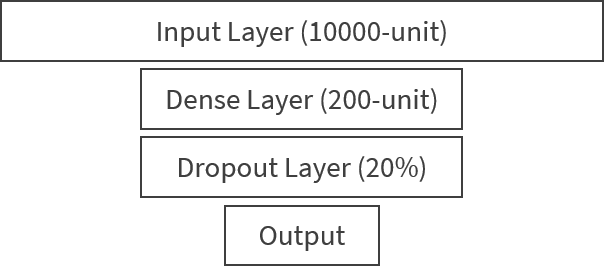
\includegraphics[width=\linewidth]{images/DeepBugs neural network.png}
%     \caption{Architecture of the DeepBugs classifier.}
%     \label{fig:deepbugs_neural_network}
% \end{figure}

% \textbf{Verification:} We will test our implementation using the authors' validation dataset. To further explore DeepBugs' generalization capabilities, we will also create our own test examples with non-JavaScript languages (in particular, other dynamically typed languages like Python and other strictly typed languages like C) and report on our findings.

% \subsection{Dissemination and continued work}
% \label{subsec:dissemination_and_continued}
% Should our project conclude successfully, we may disseminate our replication studies via the ROSE Festival. Additionally, because not every member of our team is well-versed in Python deep learning frameworks like TensorFlow, we estimate the project will take a full semester to complete. However, if we complete the work more quickly, our team plans to perform a replication study of other automated bug detection papers. Monperrus et al.'s \textit{Detecting Missing Method Calls in Object-Oriented Software} \cite{monperrus_detecting_2010} is of particular interest because in contrast to DeepBugs, that work uses hand-crafted statistical methods to find bugs.
\section{Comparing with the Original}
\label{sec:evaluating-deepbugs}

Like the original authors, we evaluate our replicated DeepBugs using switched-argument bugs identified in the 150k JavaScript Dataset \cite{raychev_learning_2016}. The dataset is already partitioned into training and evaluation categories.

First, we extract every 2-argument function call group from the ASTs generated for the dataset. Specifically, we extract every function call that fits either of the following patterns:

\begin{itemize}
    \item \texttt{functionName(arg1, arg)}
    \item \texttt{objectName.methodName(arg1, arg2)}
\end{itemize}

Note that in the second pattern, the function name is extracted for \texttt{methodName}, not \texttt{objectName.methodName}. Attempting to vectorize \texttt{objectName.methodName} would produce two vectors instead of one, because Word2Vec would need to vectorize \texttt{objectName} and \texttt{methodName} separately. The neural network has a fixed input size, so we must ensure that every extracted sample produces exactly three vectors, instead of a mix of three- and four-vector samples.

For every 2-argument function call we extract, we assume that the argument ordering is correct. Thus, the extracted function calls comprise our positive data samples. We make that assumption because the 150k JavaScript dataset is built using code from various public, open-source projects, so the source code is less likely to be buggy.

To create negative data samples, we simply switch the order of the \texttt{(arg1, arg2)} for all extracted 2-argument function calls. Thus, our training and testing data is comprised of 2$\times$ the number of extracted samples:

\begin{itemize}
    \item \texttt{functionName(arg1, arg2)} - POSITIVE
    \item \texttt{functionName(arg2, arg1)} - NEGATIVE
    \item \texttt{objectName.methodName(arg1, arg2)} - POSITIVE
    \item \texttt{objectName.methodName(arg2, arg1)} - NEGATIVE
\end{itemize}

Each data sample is then vectorized using the following procedure. Via the AST-to-Token method described in Step 2 (Sec. \ref{subsec:step-2}), we convert each data sample into a tuple of three tokens (e.g., \texttt{(``ID:functionName'', ``ID:someParam'',  ``LIT:true'')}). Each of the three tokens is individually vectorized using the Word2Vec model we trained in Step 3 (Sec. \ref{subsec:step-3}). The final, classifier-ready sample is comprised of the three vectors, concatenated into a larger vector.

To train our DeepBugs classifier from Step 4 (Sec. \ref{subsec:step-4}), we use the vectorized data samples from the 150k JavaScript dataset's training partition. Training is completed rapidly (10 epochs, batch size 100, RMSprop optimizer with binary cross-entropy loss).

As shown in Tab. \ref{tab:deepbugs-comparison}, our results are very similar to those reported by the original authors. We compare multiple aspects of the replication with the original.

\begin{table}[h]
\begin{tabular}{|c|l|l|}
\hline
\multicolumn{1}{|l|}{\textbf{Step}} & \textbf{Comparison Metric} & \textbf{Original VS Replication}                                                \\ \hline
\multirow{2}{*}{1 \& 2}             & Token vocabulary size     & Same: 9,994 VS 9,994                                                            \\ \cline{2-3} 
                                    & Extracted token values     & Identical                                                                       \\ \hline
3                                   & Generated vectors & \begin{tabular}[c]{@{}l@{}}Different\\ (authors did not provide\\ the seed)\end{tabular} \\ \hline
\multirow{2}{*}{4}                  & Training Loss              & Close: $\sim$0.002 VS $\sim$0.002                                               \\ \cline{2-3} 
                                    & Test Error                 & Close: $\sim$0.04 VS $\sim$0.06                                                       \\ \hline
\end{tabular}
\caption{On the switched-argument case from the 150k JavaScript Dataset, our DeepBugs
replication successfully captured similar performance to the original authors' work.}
\label{tab:deepbugs-comparison}
\end{table}

There are a few differences between our replication and the original, however. In the original paper, the authors claim to use a vocabulary size of 10,000 unique tokens. In actuality, the Word2Vec model they provide and the model we train both retrieve the same 9,994 tokens. We believe that this difference was merely because of rounding up the number. However, there are no significant implications of this. The vectors generated are also different; the original authors do not provide their random seed for their Word2Vec model. We verify that their method works by using the vectors as input to our DeepBugs model, hence we confirm that not having the exact same seed for the vector generation does not have significant impact on our results compared to the original author's work. Our model flags many of the bugs that the original authors' did. Our accuracy is not exactly the same; although our training loss drops to roughly 0.002, like their model, our model performs with 2\% worse accuracy.

Because our work is a replication, we do not reuse artifacts generated by the original authors. Our implementations are based on our understanding of the authors' instructions in their paper. The DeepBugs authors wrote most of their code in JavaScript, while our work exclusively uses Python. We use the same dataset to verify the authors' results. A comparison between our and the authors' implementations are shown in Tab. \ref{tab:replication-discussion}.

\begin{table}[]
\begin{tabular}{|r|l|}
\hline
\textbf{\begin{tabular}[c]{@{}r@{}}DeepBugs\\ Component\end{tabular}} & \textbf{Replication VS Original Authors}                                                                                                                                            \\ \hline
Code-to-AST                                                           & \begin{tabular}[c]{@{}l@{}}-Both use Acorn to generate ASTs\\ -Beyond that, we reimplement\\ everything in Python using our\\ own logic\end{tabular}                                \\ \hline
AST-to-Token                                                          & \begin{tabular}[c]{@{}l@{}}-We implement everything in Python\\ from scratch\end{tabular}                                                                                           \\ \hline
Token-to-Vector                                                       & \begin{tabular}[c]{@{}l@{}}-Both use the Gensim language framework\\ -We implement everything in Python\\ from scratch\end{tabular}                                                 \\ \hline
Bug Classifier                                                        & \begin{tabular}[c]{@{}l@{}}-Both use Tensorflow/Keras\\ -We implement everything in Python\\ from scratch\\ -We train the model ourselves\end{tabular}                              \\ \hline
Dataset                                                               & \begin{tabular}[c]{@{}l@{}}-Both use the 150k JavaScript Dataset\\ -Our scripts to prepare the dataset for\\ classification are reimplemented in\\ Python from scratch\end{tabular} \\ \hline
\end{tabular}

\caption{Our replication uses the same dataset and a few of the same third-party libraries as the original authors, but we implement everything else from scratch based on the instructions from the paper. We do not use any artifacts produced by the original authors.}
\label{tab:replication-discussion}
\end{table}

Because our results are very similar and were produced using artifacts that we generated ourselves, we are confident that the DeepBugs paper's results are valid; our replication is successful.
\section{Conclusions}
Although there are many tools to help software engineers identify and mitigate bugs, such as fuzzers, linters, and unit test frameworks, deep learning provides another avenue to develop tools which can support the software development process. The original DeepBugs study addressed the problem of name-based bug detection through deep learning. The study was able to produce detectors with high accuracy. Following the procedure outlined in the study, our team was able to replicate results with similar accuracy and precision. In the future, our team plans to share our results with the software engineering community by submitting the results to a suitable venue (such as the Journal of Open Source Software). To provide further insights into DeepBugs' capabilities, we currently consider to further test DeepBugs beyond the 150k JavaScript Dataset, either with a different corpus of JavaScript code or with different programming languages entirely (this will require modification of a few DeepBugs elements). Implementing DeepBugs for a variety of languages can assist software engineers in the detection of these name-based bugs and increase the quality of software across the board.


% In the original study, the target language was JavaScript to test the viability of name-based bug detection with a dynamically-typed language. In the future, similar technologies could be 

% reported differences and stuff

\section{Appendix A: Ethics Assessment}
\label{sec:appendix_a}
% Dario
\subsection{Dario}
Just as software engineers must submit their code for review to their peers, so too must the authors of research papers submit their work to the academic community. In a similar fashion, the authors offer up their work for the scrutiny of their peers to find validation. This process has ethical implications that go beyond the opinions of the reviewers. In this case, our attempt to replicate the Deepbugs study found similar results to that specified in the original study. As such, the time our group spent this semester serves to fortify the claims made in the original study and provide additional, independent proof to the validity of this work.

% Abhimanyu

\subsection{Abhimanyu}
Conducting replication and reproduction studies of previously conducted research is one of the hallmarks of good science. Reproducibility provides scientists with evidence that research results are objective and reliable and not due to bias or chance 
\cite{rooney_how_2016}. Replication and reproduction cumulatively help in addressing ethical issues such as data falsification. In this project, the team worked on implementing the work done in DeepBugs. This helped in verifying and validating results put forth by the author of DeepBugs. Fabrication of results by the authors could lead to major ethical issues.

It is noteworthy that while the original work made use of JavaScript extensively, our implementation is in Python. It is entirely possible to see different results due to difference in programming languages being used as the code written would see variation. As engineers following ACM Code of Ethics, one must be responsible and avoid public harm. The results put forth by DeepBugs along with the result validation done gives credibility to the original author's work. An automated bug detection tool like DeepBugs would certainly prove to be useful to the engineering society.

An ethically ideal software engineer would be an individual who is honest, responsible, and courageous. These aspects are crucial because these would impact the choice a software engineer makes in difficult ethical circumstances. Moreover, these traits may not be accounted by the code of ethics that most engineers are expected to follow, they essentially come from within due to the moral values one has always been bounded with. Being honest with others and towards your work is extremely important. An honest software engineer takes the responsibility and comes out to be accountable for the work done. 

Throughout our research study, we followed the ACM Code of Ethics and ensured that the replication study carried out eliminates any concerns on reproducibility. This idea ensures public welfare and ensures that no software without a strong fundamental foundation and improper testing is not proposed for public use. 

% Caleb

\subsection{Caleb}
A replication study lends credibility to an existing piece of research. In our case, we validated the results of the DeepBugs paper. By reimplementing the original authors' work entirely in Python (they used JavaScript as well), we provided more ways for the public to use the paper, making it even more accessible. Although this does support aspects of the ACM/IEEE Code of Ethics -- we help ensure that the authors stay honest with the public -- there is another ethical consideration: is the original work something that deserves the credibility we give it via replication?

I believe the original DeepBugs paper is a good contribution to science and engineering. By automating new types of bug detection, the paper provides another tool for engineers to use in their ongoing war against defects in software. Further, I find it difficult to imagine any lasting ramifications of the paper that would violate any point of the Code of Ethics. Therefore, I find this paper to be worthy of elevating via replication.

% Young
\subsection{Young} Replication and reproduction studies are essential to keep the research community healthy and reliable, by primarily allowing the other researchers to adopt, verify and possibly extend the implementation with confidence. As noted earlier, the community recognizes this as a ``reproducibility crisis.''
An ethically ideal person is courageous without manifesting the common virtue or excellence to the maximum extent possible, beyond what’s ordinary. Harris Jr. describes this as a ``virtue portrait'' in his article. \cite{harris_good_2008}
With the technical and non-technical excellence, one can attempt to sketch a virtue portrait of the ethically ideal software engineer. It is our belief that all software engineers should attempt to picture virtue portrait on themselves while practicing software engineering especially by contemplating and possessing an utmost interest in the social outcome of one's action. We believe that our practice of replication helps mitigate the reproducibility crisis and has positive ethical social outcomes by addressing the following clauses of ACM-IEEE Code of Ethics: \textit{1.03. Approve software only if they have a well-founded belief that it is safe, meets specifications, passes appropriate tests, and does not diminish the quality of life, diminish privacy or harm the environment. The ultimate effect of the work should be to the public good.} and \textit{3.10. Ensure adequate testing, debugging, and review of software and related documents on which they work.} 

% Jordan

\subsection{Jordan}
Replication and reproduction studies are part of healthy scientific progress. Repeatability of observation is a core part of the scientific method. The scientific method has been a staple formula for both the natural and social sciences since its inception. Reproduction studies are also important in the formal sciences. In the formal sciences, it is more so called publishing an alternate proof, instead of a reproduction study. In the formal sciences, it is important to do this for sake of understanding the result from a different perspective. It is also the case that results in formal sciences, if complex enough, may disagree. \cite{lipton_social_1979} Replication is often done ``automatically'' as a result of re-creating a proof when one reads a paper. But having multiple alternate published proofs adds confidence in the correctness of a result.

\iffalse
% ethical word fodder below: MIT licensed
DeepBugs falls into the category of being both an empirical scientific result and a formal one. Although computer science is categorized as part of the formal sciences, Artificial Intelligence methods which involve learning, are potentially different from this categorization. This is due to the fact that learning methods can use empirical data. And so, for a machine learning algorithm such as DeepBugs, behavior can be different under a different set of data. 
% Also note the attempt at replication of 150 DNN's here
As a formal result, DeepBugs uses a particular implementation with JavaScript and Python. The result could be different if implemented using different code. That is not say there are any issues with Python and JavaScript in particular, or programming skills of the researchers from the previous paper. The choice is not due to recent statistical analysis on programming languages versus problem domains. \cite{berger_impact_2019,ray_large_nodate}
The aim instead is to implement a solution in a different way, because it is different. And Python and TensorFlow in particular are chosen because our group's skills mostly overlap on these tools. 


There are also ethical concerns for robustness of this research for use in engineering. By the ACM code of ethics, we must avoid harm. \cite{noauthor_code_2016} The result from DeepBugs, and results of similar impact, should be used in a way that minimizes harm. Replication of results increases confidence in those results, before they are used in products that effect people. Replication of results also follows the ethical standard that engineers should strive to be honest and trustworthy. Ignoring due diligence to replicate results for sake of personal gain is at the cost of people that rely on these results.


%% covered several times in above sections
% A successfully replicated study will confirm the result from DeepBugs. Extensions to DeepBugs can be made with higher confidence of correctness. A negative result will draw attention to any potential weaknesses in the methodology from either this paper or the original, encouraging refinement on the result from DeepBugs. 

%import Code_of_Ethics_for_Engineers 

\fi


\section{Appendix B: Artifacts}
Our code is version-controlled on GitHub. We provide a README and commented code 
at \url{https://github.com/code-correctional-facility/deepbugs-jr}.

\iffalse
\label{sec:appendix_b}
The purpose of our project is to reproduce the DeepBugs study to substantiate the authors' claim  of name-based bug detection through machine learning. To do so, we will follow the study's approach to using a TensorFlow machine learning model. Our team has set up a repository on Github where our project will be hosted and tracking tasking through a kanban board on Jira. The team will proceed to assess the requirements specified in the study. Once completed, we will begin compiling tasks for the project backlog. At this stage, development of the neural network layers will commence. 

As explained in Section \ref{sec:timeline}, our team will use Scrum for day-to-day operations. However, we do plan to create most of the requirements at the start of the project and follow the macro flow process shown in Figure \ref{fig:engineering_process}.

\begin{figure}[ht]
    \centering
    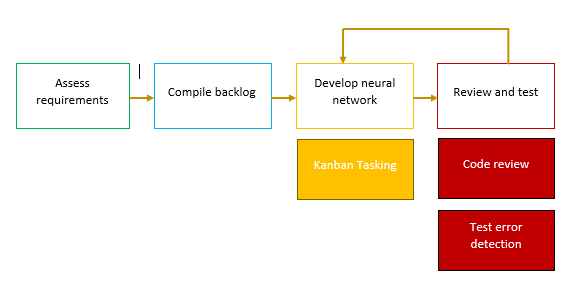
\includegraphics[width=\linewidth]{images/Engineering Process.PNG}
    \caption{Project Flow Overview}
    \label{fig:engineering_process}
\end{figure}

Our team has established a scheduled meeting on a weekly basis which will be used to assign tasks and provide status updates for work in progress. In the spirit of following suit with \textit{Software Engineering at Google}'s approach to code review, we will require changes to source code receive a "looks good to me" from any other member of the team.

Lastly, relevant works used in the development of our reproduction will be tracked in Zotero. This tool will allow the team to maintain a list of works which will be cited as resources.

\fi
% post mortem

\section{Appendix C: Post Mortem}

% \subsection{Our Proposal VS Our Actual Work}
% \label{subsec:our-proposal-vs-our-actual}


\subsection{What Went Well}
The team largely feels that the project went smoothly. The replication was completed successfully, and the team gelled well and operated without conflicts.

\subsubsection{\textbf{We intentionally and carefully designed procedures for effectively producing code, and stuck to them throughout our project.}} At the start of the project, our team clearly laid out procedures for checking code into Git, writing unit tests, conducting code reviews, and communicating with Teams. We established an automated Kanban board and issue tracker, and we maintained a steady backlog of tasks to draw from.

\subsubsection{\textbf{We planned for success!}} We spent a considerable amount of time identifying tasks from the original DeepBugs paper. By conducting a comprehensive review of the process followed by the authors, we were able to identify the major milestones necessary for completing the project. The team went on to further break down each of the milestones into a list of actionable items which would ultimately become the backlog the team used to plan out the replication. This allowed the development process to move along smoothly. During our weekly check-in meetings the team would view the board with this list and easily understand what was in progress and what the next steps were once tasks were completed.

\begin{figure}[h]
    \centering
    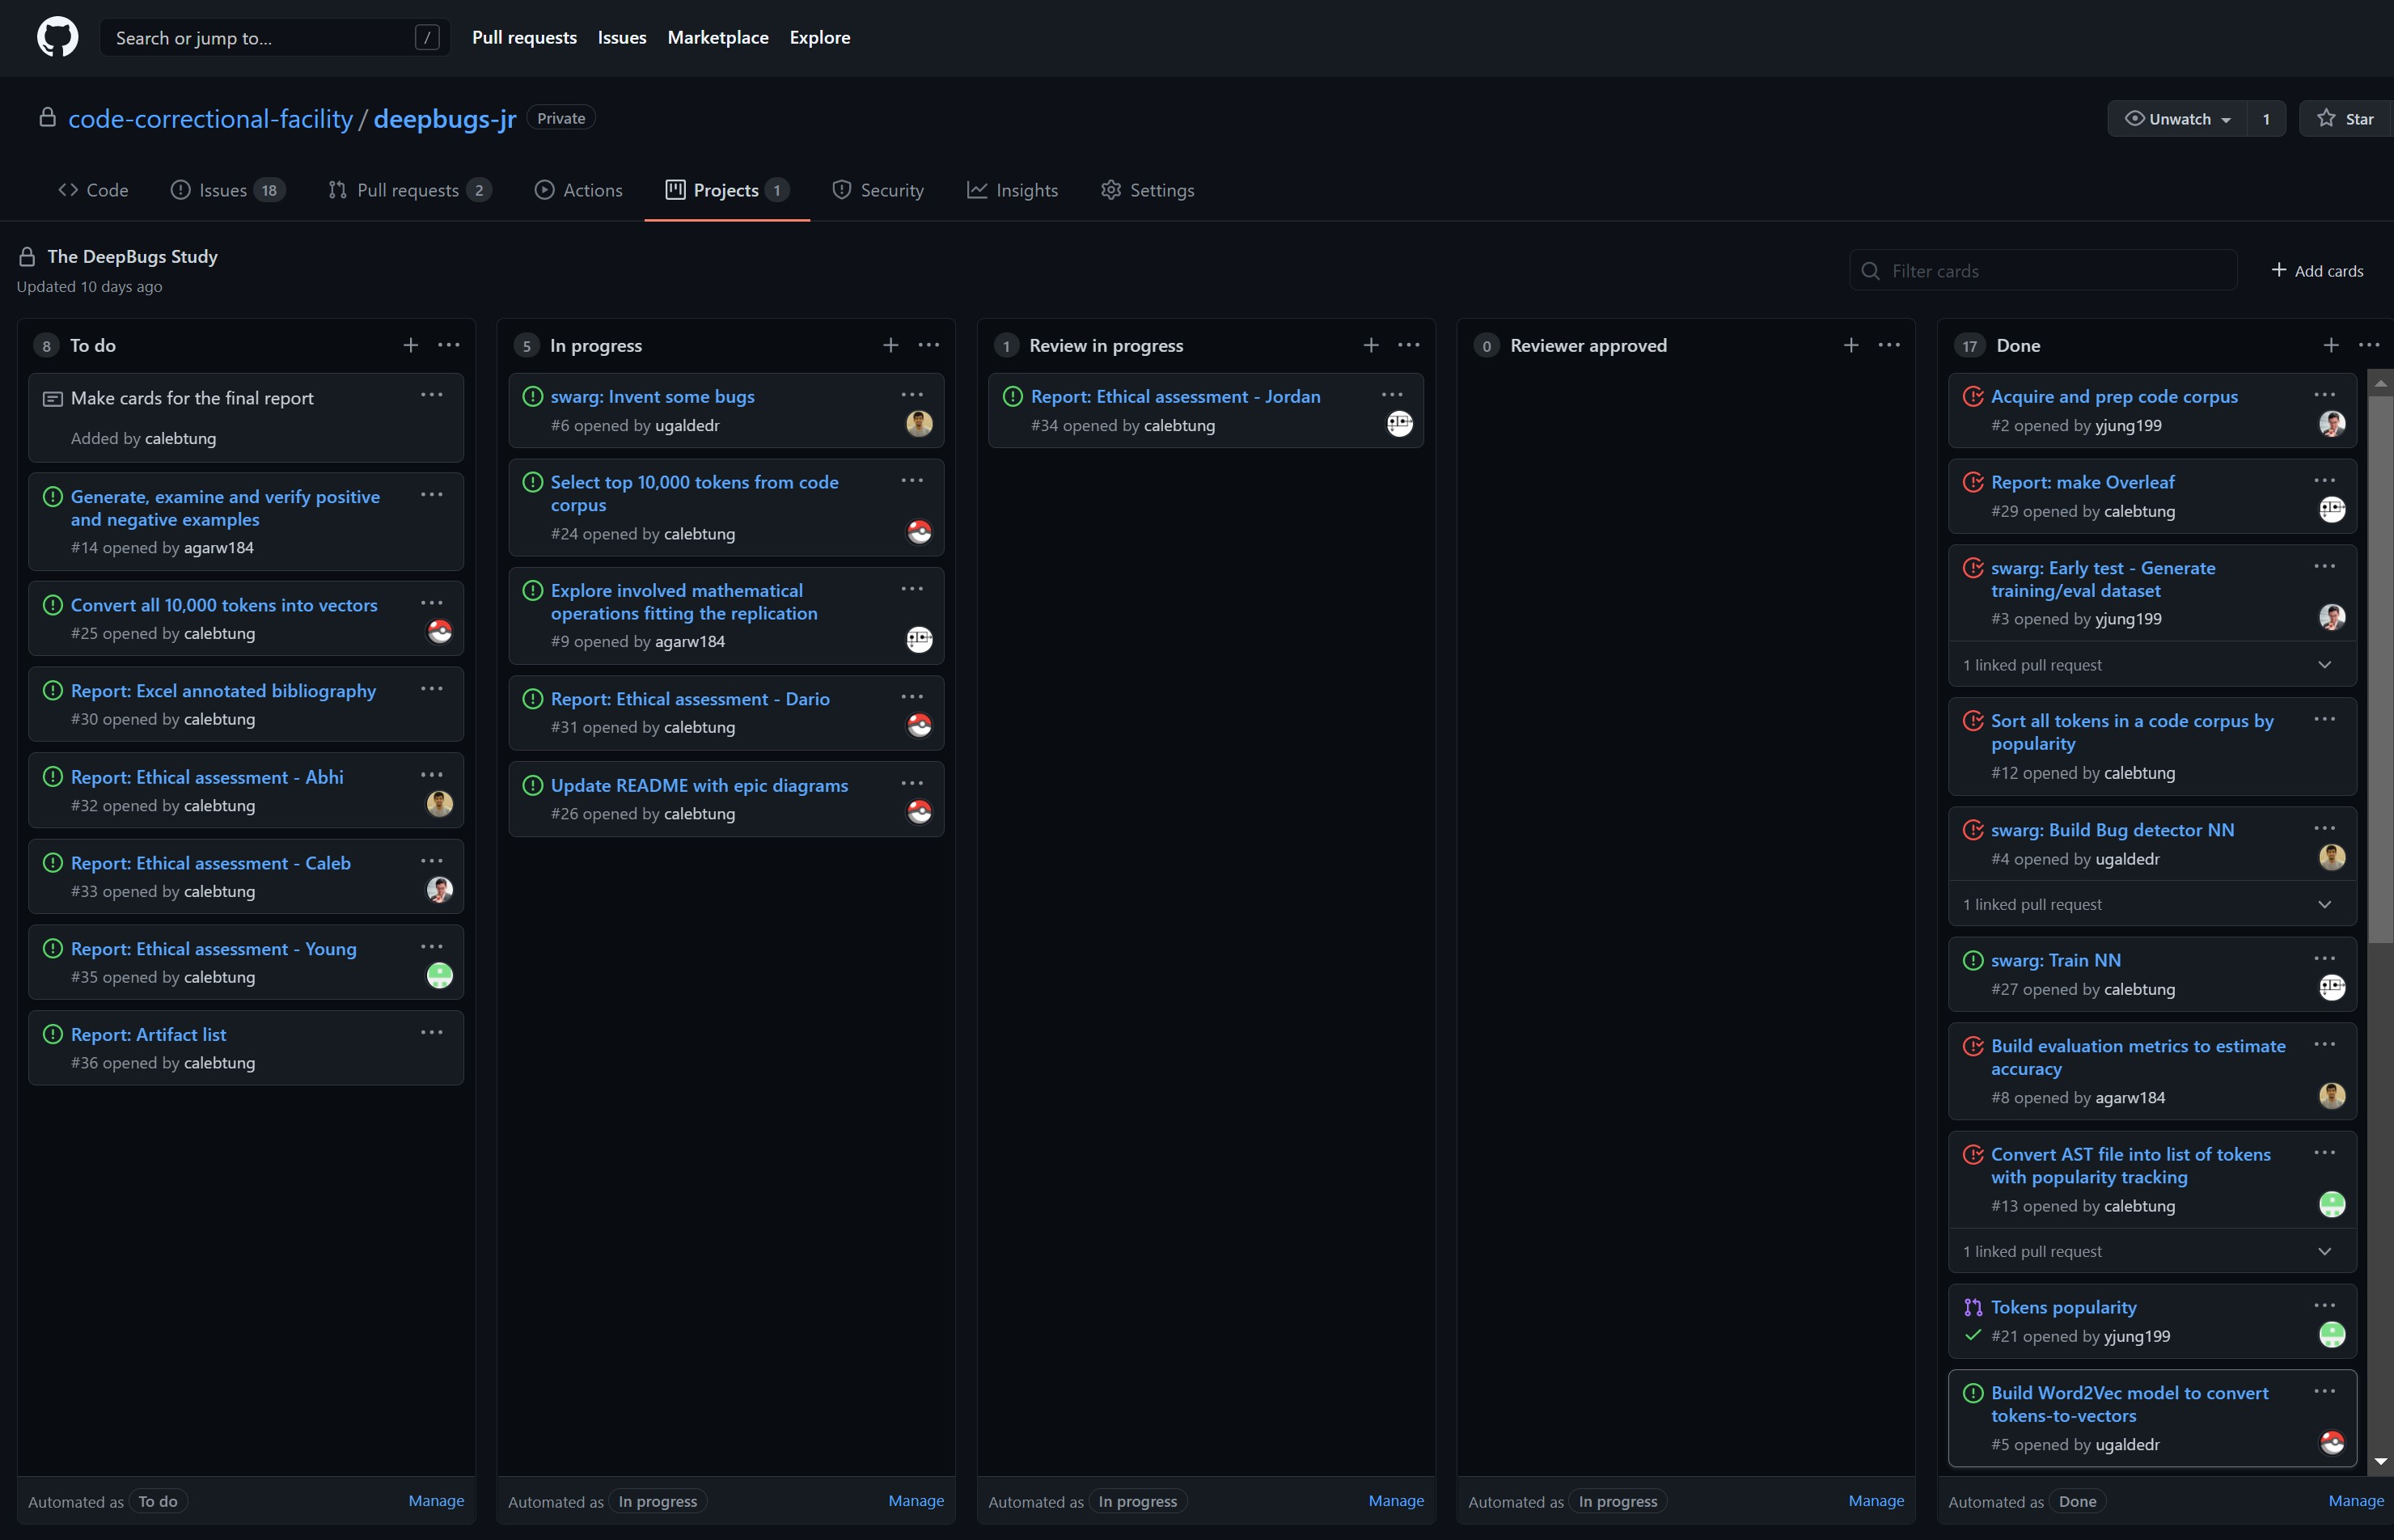
\includegraphics[width=\linewidth]{images/GitHub Projects.jpg}
    \caption{Example of our kanban board with automated issue tracking. As we completed pull requests, the cards automatically rearranged themselves on the board.}
    \label{fig:github-projects}
\end{figure}

\subsubsection{\textbf{Our team collaborated productively.}} Several tasks on the backlog were completed by multiple members working closely together. Although we were careful to assign tasks in bite-sized chunks to stay quasi-Agile, some tasks wound up requiring more assignees. Team members would help each other by pair programming and recommending additional resources. The team did an excellent job of keeping each other in the loop when faced with any issues. This was accomplished by using Microsoft Teams as a general chat. Members would regularly ping the rest of team to ask for advice or alert others on the completion of tasks. The members were highly responsive and received feedback within a matter of minutes in most cases. We all performed manual code reviews to stay familiar with our codebase and ``enforce'' good practices through peer pressure.

\subsubsection{\textbf{We stayed on schedule, with room for flexibility.}} With our team spread across the globe (multiple US timezones and South Korea), we designed our workflow asynchronously, supplemented with regular, synchronous ``tag-up'' meeting times. By investing effort in maintaining a granular, bite-sized backlog, we kept work from getting bottlenecked by members needing to communicate across 13-hour time gaps. US members maintained empty slots in their evening schedules and Korea members kept their mornings open, allowing us to accommodate the few time it was necessary to synchronize outside of meeting time. Our project was thus able to adhere to our schedule, without demanding excessive commitments from team members.

\subsubsection{\textbf{We developed camaraderie.}} No one on the team had met each other prior to the project. By keeping our meetings casual and cracking jokes, the team successfully established a pleasant working environment that was able to complete the project without the usual ``storming'' period of team development.

\subsubsection{\textbf{We produced quality, useful software.}} We created well-documented, test-covered software: an easy-to-use replication of the DeepBugs paper. This would provide more options to users looking to try out the DeepBugs framework (the original authors used mostly JavaScript, but all of our code was written in Python).

\subsubsection{\textbf{We became better engineers.}} Not only was this project a terrific opportunity for us all to gain technical competency in an area of research that we had never dealt with before, but it also allowed us to exercise other software engineering muscles. In order to better understand some of the modern tools used in the software development process, our team set up our Github repository to make use of Github Actions any time code was pushed. This provided members of the team who were not familiar with the typical continuous integration process insight as to how to define and implement a continuous integration pipeline. Building on the development operations process, the python unittest module along with a basic smoke test were implemented to demonstrate a continuous integration pipeline for our project. This allowed members put material discussed earlier in the semester to practical use. We agreed to add tests for branching points to provide coverage as well as, edge cases to ensure proper functionality in the code. In the future, this project could possibly serve as reference material should any team member be required to go through setting up similar infrastructure once again.  


\subsection{What Did Not Go So Well}
Although the project was completed successfully, our team did run into an unanticipated roadblock in the middle of development.


%From SE @ Google: ``A good postmortem should include the following:

%A brief summary of the event

%A timeline of the event, from discovery through investigation to resolution

%The primary cause of the event

%Impact and damage assessment

%A set of action items (with owners) to fix the problem immediately

%A set of action items to prevent the event from happening again

%Lessons learned''

\subsubsection{\textbf{Almost bit off more than we could chew.}} Prior to the project proposal, our team had a very different vision of what our project would look like. Originally, the team had planned to conduct a systemic review on the state-of-art of automated software testing research. In addition to this, the team envisioned the creation of a tool which could direct software engineers to a variety of testing applications intended for the identification of specific bugs. After discussion with Professor Davis following the proposal, the team was reigned in and the scope of the project was narrowed to this replication. It was unfortunate that correcting the team onto this path ate some of the initial planning time leading up to the first status update. In hindsight, now that we've completed our replication, it is quite clear completing a systemic review, generating a tool based on our findings, and compiling this report would not have been feasible within this time frame.

\subsubsection{\textbf{Losing time for 10,000 tokens.}} During the course of development, our team encountered an unnecessary time sink while parsing tokens for training the Word2Vec model. Dario and Young had been assigned tasks to collect the top 10,000 tokens from the source code dataset and train the Word2Vec model. Even after the two spent a week and many precious development hours on the method, the model was still not functioning correctly. After this was brought up during the weekly team meeting, the rest of the team moved to assist, conducting code reviews and familiarizing themselves with the Word2Vec paper. While browsing documentation online, Caleb discovered that the team's desired functionality was actually already implemented in the Word2Vec model framework and could be activated with a single parameter. We wound up discarding the additional code written over the week in favor of this simpler solution. This unfortunate situation could have been avoided by spending a little more time understanding the tools we used for the study. The issue cost the team valuable hours which could have been better spent supporting other tasks. Ultimately, the task was still resolved according to schedule, but any possible time savings were lost. Going forward, scheduling time to do documentation reviews for the tools being used could prevent these types of situations. 


% \section{Introduction}
% ACM's consolidated article template, introduced in 2017, provides a
% consistent \LaTeX\ style for use across ACM publications, and
% incorporates accessibility and metadata-extraction functionality
% necessary for future Digital Library endeavors. Numerous ACM and
% SIG-specific \LaTeX\ templates have been examined, and their unique
% features incorporated into this single new template.

% If you are new to publishing with ACM, this document is a valuable
% guide to the process of preparing your work for publication. If you
% have published with ACM before, this document provides insight and
% instruction into more recent changes to the article template.

% The ``\verb|acmart|'' document class can be used to prepare articles
% for any ACM publication --- conference or journal, and for any stage
% of publication, from review to final ``camera-ready'' copy, to the
% author's own version, with {\itshape very} few changes to the source.

% \section{Template Overview}
% As noted in the introduction, the ``\verb|acmart|'' document class can
% be used to prepare many different kinds of documentation --- a
% double-blind initial submission of a full-length technical paper, a
% two-page SIGGRAPH Emerging Technologies abstract, a ``camera-ready''
% journal article, a SIGCHI Extended Abstract, and more --- all by
% selecting the appropriate {\itshape template style} and {\itshape
%   template parameters}.

% This document will explain the major features of the document
% class. For further information, the {\itshape \LaTeX\ User's Guide} is
% available from
% \url{https://www.acm.org/publications/proceedings-template}.

% \subsection{Template Styles}

% The primary parameter given to the ``\verb|acmart|'' document class is
% the {\itshape template style} which corresponds to the kind of publication
% or SIG publishing the work. This parameter is enclosed in square
% brackets and is a part of the {\verb|documentclass|} command:
% \begin{verbatim}
%   \documentclass[STYLE]{acmart}
% \end{verbatim}

% Journals use one of three template styles. All but three ACM journals
% use the {\verb|acmsmall|} template style:
% \begin{itemize}
% \item {\verb|acmsmall|}: The default journal template style.
% \item {\verb|acmlarge|}: Used by JOCCH and TAP.
% \item {\verb|acmtog|}: Used by TOG.
% \end{itemize}

% The majority of conference proceedings documentation will use the {\verb|acmconf|} template style.
% \begin{itemize}
% \item {\verb|acmconf|}: The default proceedings template style.
% \item{\verb|sigchi|}: Used for SIGCHI conference articles.
% \item{\verb|sigchi-a|}: Used for SIGCHI ``Extended Abstract'' articles.
% \item{\verb|sigplan|}: Used for SIGPLAN conference articles.
% \end{itemize}

% \subsection{Template Parameters}

% In addition to specifying the {\itshape template style} to be used in
% formatting your work, there are a number of {\itshape template parameters}
% which modify some part of the applied template style. A complete list
% of these parameters can be found in the {\itshape \LaTeX\ User's Guide.}

% Frequently-used parameters, or combinations of parameters, include:
% \begin{itemize}
% \item {\verb|anonymous,review|}: Suitable for a ``double-blind''
%   conference submission. Anonymizes the work and includes line
%   numbers. Use with the \verb|\acmSubmissionID| command to print the
%   submission's unique ID on each page of the work.
% \item{\verb|authorversion|}: Produces a version of the work suitable
%   for posting by the author.
% \item{\verb|screen|}: Produces colored hyperlinks.
% \end{itemize}

\printbibliography

\end{document}
